%! Author = Ivan Chizhov
%! Date = 08.11.2022

% Preamble
\documentclass[colorthm]{../civarticle}
\usepackage[math]{blindtext}

\title{
    Потоковые шифры. Шифр SEAL\\
    %\small{(оформление окружений цветом и пр.)}%
}
\author{А.~С.~Сахаутдинова}
\if 0
\abstract{%
    \Blindtext[2][1]
}
\keywords{%
    \Blindtext[1][1]
}
\fi
% Document
\begin{document}
\blindmathtrue
\section{Введение}
\label{sec:thm-pif}

В современном мире, где безопасность данных становится все более критическим аспектом информационных технологий, криптография играет ключевую роль в защите конфиденциальности и целостности информации. Одним из наиболее важных и широко используемых классов криптографических алгоритмов являются потоковые шифры. Они отличаются от блочных шифров своей способностью шифровать цифровые данные бит за битом или байт за байтом, что делает их идеальными для работы с большими объемами данных в режиме реального времени.

Это эссе посвящено изучению и анализу различных потоковых шифров, каждый из которых внес свой уникальный вклад в область криптографической безопасности. Мы рассмотрим такие шифры, как RC4, известный своей простотой и скоростью, Snow3G, широко применяемый в сотовой связи, LILI-128, предлагающий уникальный механизм обратной связи, SEAL, отличающийся высокой производительностью, MUGI, который получил распространение в Японии, а также шифры семейства A5 (A5/1, A5/2, A5/3), используемые в GSM сетях.

Особое внимание в данной работе уделяется шифру SEAL. Этот шифр демонстрирует уникальное сочетание скорости и безопасности, что делает его привлекательным для множества приложений. Тем не менее, как и большинство криптографических систем, SEAL подвержен определенным видам атак, анализ которых имеет важное значение для понимания и улучшения криптографических протоколов.

\section{Термины и определения}

\textbf{Зашифрование}: Обратимое преобразование данных с помощью шифра, которое формирует шифртекст из открытого текста.

\textbf{Ключ}: Изменяемый параметр в виде последовательности символов, определяющий криптографическое преобразование.

\textbf{Открытый текст}: Незашифрованная информация.

\textbf{Потоковый шифр}: Шифр из класса симметричных криптографических методов,в котором каждый символ открытого текста преобразуется в символ шифртекста в зависимости не только от используемого ключа, но и от его расположения в потоке открытого текста.

\textbf{Расшифрование}: Операция, обратная к зашифрованию.

\textbf{Симметричный криптографический метод}: Криптографический метод, использующий один и тот же ключ для преобразования, осуществляемого отправителем. и преобразования, осуществляемого получателем.

\textbf{Шифр}: Криптографический метод, используемый для обеспечения конфиденциальности данных, включающий алгоритм зашифрования и алгоритм расшифрования.

\textbf{Шифртекст}: Данные, полученные в результате зашифрования открытого текста в целях скрытия его содержания.


\section{Описание шифров}

\begin{enumerate}
\item \textbf{RC4 ~\cite{RC4} }

\textit{Описание}: RC4 - это широко используемый поточный шифр, характеризующийся простотой и скоростью. Он был разработан Роном Ривестом в 1987 году. RC4 генерирует псевдослучайный поток ключей, который затем комбинируется с открытым текстом.

\textit{Схема и Устройство}: В основе RC4 лежит таблица перестановок, которая инициализируется секретным ключом, и затем используется для генерации ключевого потока. Это достигается с помощью операций перестановки и замены.

\textit{Функции}: Главной функцией RC4 является генерация ключевого потока, который имеет высокую энтропию и используется для шифрования данных.


\item \textbf{Snow3G ~\cite{snow} }

\textit{Описание}: Snow3G - это поточный шифр, разработанный для использования в стандартах UMTS и LTE. Он был выбран как основа для алгоритмов шифрования и целостности данных в этих сетях.

\textit{Схема и Устройство}: Snow3G использует комбинацию линейного сдвигового регистра и нелинейной функции обработки. Это обеспечивает высокую степень безопасности и производительности.

\textit{Функции}: Основная функция Snow3G - обеспечение шифрования и целостности данных в сетях мобильной связи.



\item \textbf{LILI-128 ~\cite{lili} }

\textit{Описание}: LILI-128 - это поточный шифр, основанный на использовании регистров сдвига с линейной обратной связью (LFSR). Он был разработан для обеспечения высокой стойкости к криптоаналитическим атакам.

\textit{Схема и Устройство}: Шифр состоит из двух LFSR различной длины, которые работают вместе для генерации ключевого потока.

\textit{Функции}: LILI-128 предназначен для защиты данных путем генерации сложного ключевого потока, который трудно анализировать.


\item \textbf{SEAL}

\textit{Описание}: SEAL (Software-Optimized Encryption Algorithm) - это поточный шифр, оптимизированный для программной реализации. Он разработан для машин с 32-битным размером слова и обширной оперативной памятью.

*\textit{Схема и Устройство}: SEAL является семейством псевдослучайных функций, способным генерировать произвольные части ключевого потока.

\textit{Функции}: Основной функцией SEAL является обеспечение высокоскоростного шифрования с возможностью легкой генерации различных частей ключевого потока.


\item \textbf{MUGI ~\cite{Mugi} }

\textit{Описание}: MUGI - это японский поточный шифр, разработанный для 64-битных архитектур. Он использует 128-битный мастер-ключ и 128-битный вектор инициализации.

\textit{Схема и Устройство}: MUGI основан на большом нелинейном регистре сдвига обратной связи (NLFSR) и дополнительном нелинейном состоянии.

\textit{Функции}: Шифр предназначен для обеспечения безопасности данных, используя сложные алгоритмы обновления состояния.

\item \textbf{Шифры семейства A5 ~\cite{A5} }

\textit{Описание}: Семейство шифров A5 включает A5/1, A5/2 и A5/3. Эти шифры используются для шифрования воздушных передач в стандарте GSM.

\textit{Схема и Устройство}: Шифры A5 комбинируют несколько линейных регистров сдвига с обратной связью (LFSR), чьи такты управляются некоторыми из их битов.

\textit{Функции}: Основная функция шифров семейства A5 - обеспечение конфиденциальности и целостности данных в сетях мобильной связи.

\end{enumerate}


\section{Шифр SEAL}

Шифр SEAL (Software-Optimized Encryption Algorithm) был разработан в IBM Филом Рогэвем и Доном Копперситом в 1993 году. Алгоритм оптимизирован для 32-битных процессоров. ~\cite{Handbook}


\subsection{Технические характеристики}

\textbf{Стартовые условия}: кэш-память на несколько килобайт и восемь 32-битных регистров.

\textbf{Длина ключа}: 160 бит;

\textbf{Алгоритм}: (Описание алгоритма основано на ~\cite{SHnaier} ) Шифр SEAL представляет собой семейство псевдослучайных функций. Для того, чтобы не было нежелательных потерь скорости из-за медленных операций обработки ключа, шифр SEAL выполняет с ним рядо предварительных действий, сохраняя результаты в трех таблицах: R, S и T. Эти таблицы испольузются для ускорения шифрования и дешифрования. 

Предварительная обработка отображает ключ k на эти таблицы с помощью процедуры, основанной на SHA.

Также SEAL использует четыре 32-битовых регистра, А, В, С и D, начальные значения которых определяются n и полученными по k таблицами R и Т. Данные регистры изменяются в ходе итераций, каждая из которых состоит из восьми этапов. На каждом этапе 9 битов первого регистра (A, B, C или D) используются в качестве индекса таблицы Т. Затем выбранное из T значение складывается со вторым регистром (A, B, C или D) или объединяется с его содержимым с помощью XOR. Потом первый регистр циклически сдвигается на 9 позиций. На некоторых этапах второй регистр далее модифицируется с помощью сложения или XOR с содержимым первого регистра (уже сдвинутым). После 8 таких этапов А, В, С и D добавляются к потоку ключей, при этом каждый из них маскируется сложением или XOR с определенным словом из S. Итерация завершается прибавлением к А и С дополнительных значений, зависящих от $n_1, n_2, n_3, n_4)$ , выбор конкретного значения определяется четностью номера итерации.

Внутренний цикл SEAL представлен на Рис.1.

\begin{figure}[h]
{
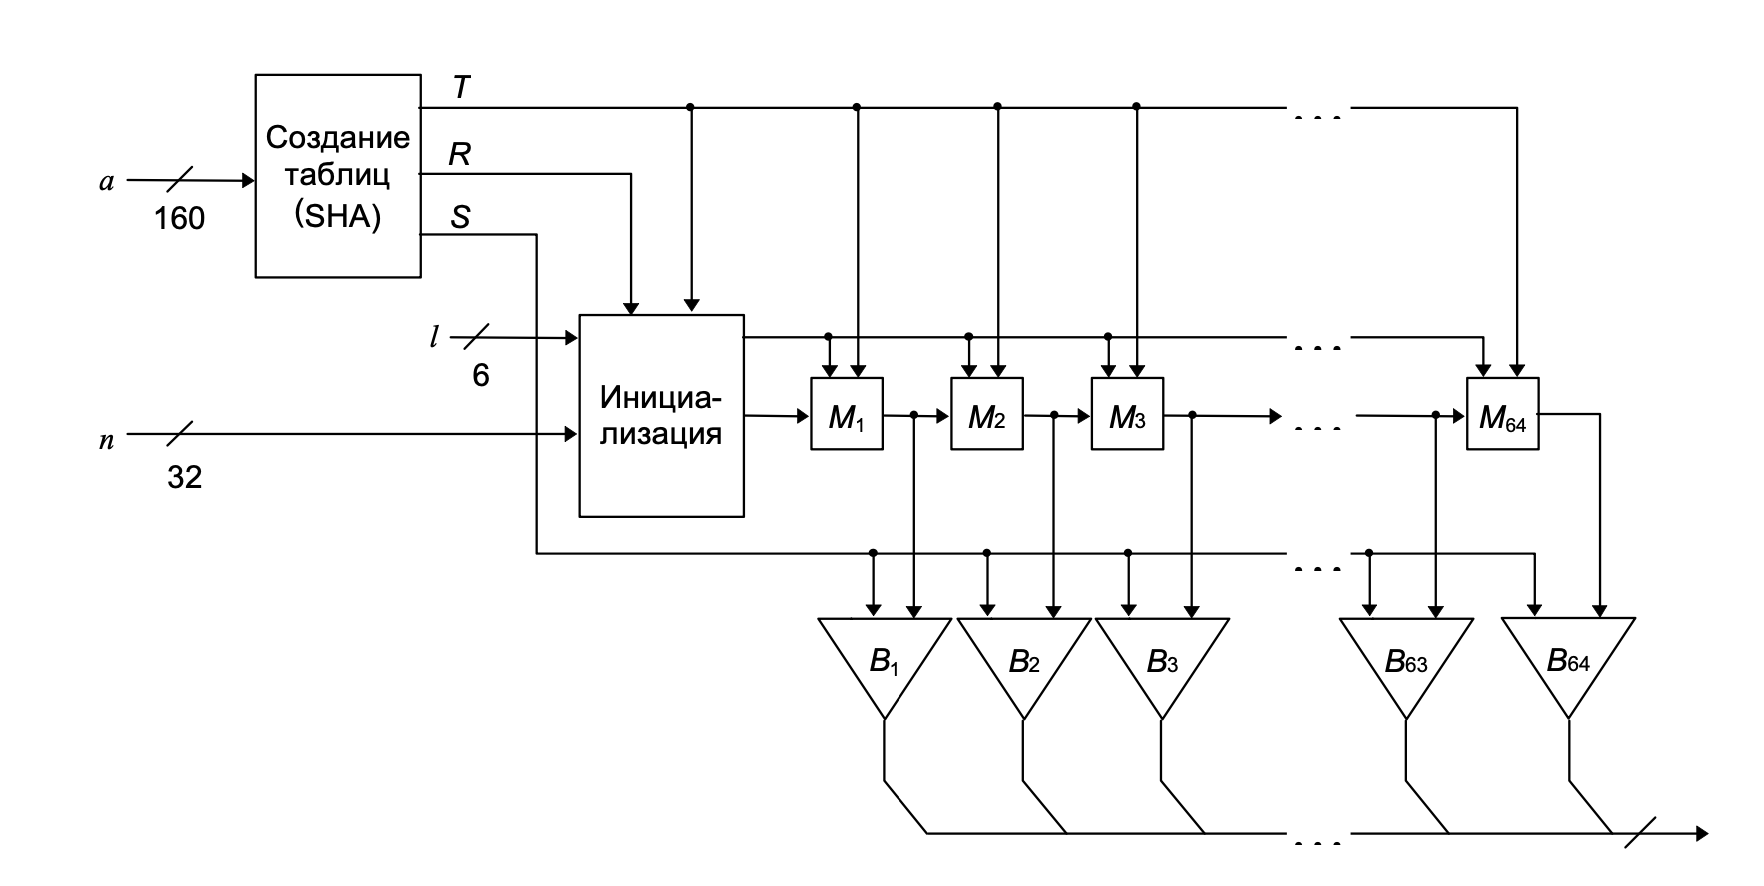
\includegraphics[width=0.99\linewidth]{example/SEAL.png} } 

\caption{Внутренний цикл SEAL}
\end{figure}

\subsection{Эксплуатационные характеристики}

\textbf{Скорость шифрования}: примерно 4 машинных такта на байт текста;

\textbf{Преимущества}: Так как SEAL является семейством псевдослучайных функций, он удобен в ряде случаев, где неприменимы традиционные потоковые шифры. При использовании большинства потоковых шифров, создается однонаправленная опоследовательность битов. В таком случае i-ый бит можно определить только сгенерировав все биты до i-го. В случае с SEAL можно получить доступ к любой позиции потока ключей. Семейство псевдослучайных функций также упрощает проблему синхронизации. 


\textbf{Программная реализация, скорость работы}: на 50-мегагерцовом процессоре i486 скорость работы 58 Мбит/с.

\subsection{Атака на упрощенную версию SEAL 1.0 и на сам SEAL 1.0}


 В 1996 году Хелен Хандшух и Henry Gilbert описали атаки на упрощенную версию SEAL 1.0 (Все операции $+$ заменены на ХOR) и на сам SEAL 1.0. ~\cite{atack}

\textbf{Реализуемая угроза}: нахождение зависимости псевдослучайной функции от ключа. 

\textbf{Оценка числа операций}: 230 текстов, каждый длиной в четыре 32-битных слова.
 
\textbf{Пути нейтрализации атаки}: В следующих версиях алгоритма SEAL 3.0 и SEAL 2.0 были сделаны некоторые доработки и изменения. Например, в версии 1.0 каждая итерация с ключевой последовательностью завершалась модификацией только двух регистров, а в версии 3.0 — модифицировались все четыре. Ещё SEAL 3.0 и SEAL 2.0 использовали для генерации таблиц алгоритм SHA-1 вместо первоначального SHA, что сделало их более устойчивыми к криптоанализу. \href{https://ru.wikipedia.org/wiki/%D0%A5%D0%B0%D0%BD%D0%B4%D1%88%D1%83%D1%85,_%D0%A5%D0%B5%D0%BB%D0%B5%D0%BD#%D0%90%D1%82%D0%B0%D0%BA%D0%B0_%D0%BD%D0%B0_SEAL}{Википедия}.


\section{Заключение}


В результате анализа потокового шифра SEAL, можно сформулировать ряд выводов относительно его эксплуатационных аспектов, криптографической устойчивости и практического применения: 

Шифр SEAL отличается высокой скоростью обработки и оптимизирован для программных реализаций.

С точки зрения криптографической стойкости, рассмотренный шифр показывает хорошие результаты против известных методов криптоанализа. 

Таким образом, SEAL представляет собой высокоэффективный и надежный потоковый шифр, сочетающий в себе продвинутую скорость обработки и значительную криптографическую устойчивость. Однако, учитывая динамично развивающийся характер криптографической среды, необходимо обеспечить его непрерывное обновление и адаптацию для поддержания соответствующего уровня защиты данных в долгосрочной перспективе.


\label{sec:minted}
% \show\MINTED
\if \MINTED\empty
% do nothing, minted is off
\else \inputminted{python}{code.py} \fi
\end{document}
%%% Local Variables:
%%% mode: latex
%%% TeX-master: t
%%% End:
